\documentclass{urdpl}     % praca w języku polskim

% Lista wszystkich języków stanowiących języki pozycji bibliograficznych użytych w pracy.
% (Zgodnie z zasadami tworzenia bibliografii każda pozycja powinna zostać utworzona zgodnie z zasadami języka, w którym dana publikacja została napisana.)
\usepackage[english,polish]{babel}

% Użyj polskiego łamania wyrazów (zamiast domyślnego angielskiego).
\usepackage{polski}

\usepackage[utf8]{inputenc}

% dodatkowe pakiety

\usepackage{mathtools}
\usepackage{amsfonts}
\usepackage{amsmath}
\usepackage{amsthm}
\usepackage[hidelinks]{hyperref}
\usepackage{float}
\usepackage{listings}
\usepackage{graphicx}
\usepackage{subcaption}
\usepackage{booktabs} % Dla \toprule, \midrule, \bottomrule
\usepackage{multirow} 
\usepackage{tabularx} 
\usepackage{amssymb} 
\usepackage{listings}
\usepackage{xcolor}
\usepackage{array}
\usepackage{makecell}
\usepackage[flushleft]{threeparttable}
\usepackage[normalem]{ulem}
\usepackage{lineno}
\usepackage{makecell} %
\usepackage{csquotes}
\usepackage{courier}

% ------------------------
% --- < listingi > ---

\usepackage{listings}
\lstloadlanguages{TeX}
\renewcommand{\lstlistlistingname}{Spis listingów}
\renewcommand{\lstlistingname}{Listing}

\lstset{
	literate={ą}{{\k{a}}}1
           {ć}{{\'c}}1
           {ę}{{\k{e}}}1
           {ó}{{\'o}}1
           {ń}{{\'n}}1
           {ł}{{\l{}}}1
           {ś}{{\'s}}1
           {ź}{{\'z}}1
           {ż}{{\.z}}1
           {Ą}{{\k{A}}}1
           {Ć}{{\'C}}1
           {Ę}{{\k{E}}}1
           {Ó}{{\'O}}1
           {Ń}{{\'N}}1
           {Ł}{{\L{}}}1
           {Ś}{{\'S}}1
           {Ź}{{\'Z}}1
           {Ż}{{\.Z}}1,
	basicstyle=\footnotesize\ttfamily,
}

% defninicja stylu python
\lstdefinestyle{stylePython}{
    language=Python,
    commentstyle=\color{green},          % Kolor komentarzy
    keywordstyle=\color{blue},           % Kolor słów kluczowych
    numberstyle=\tiny\color{gray},       % Kolor i styl numerów linii
    stringstyle=\color{red},             % Kolor ciągów znaków
    basicstyle=\ttfamily\footnotesize,   % Podstawowy styl kodu
    breakatwhitespace=false,             % Automatyczne dzielenie wierszy
    breaklines=true,                     % Dzielenie długich linii
    keepspaces=true,                     % Zachowanie spacji
    numbers=left,                        % Numery linii po lewej
    numbersep=5pt,                       % Odstęp numerów od kodu
    showspaces=false,                    % Nie pokazuj spacji
    showstringspaces=false,              % Nie pokazuj spacji w ciągach znaków
    showtabs=false,                      % Nie pokazuj tabulacji
    tabsize=2                            % Rozmiar tabulacji
}

% defnicja stylu JAVA
\lstdefinestyle{javaStyle}{
    language=Java,
    basicstyle=\ttfamily\footnotesize,
    keywordstyle=\color{blue},
    commentstyle=\color{green!50!black}\itshape,
    stringstyle=\color{green},
    numberstyle=\tiny\color{gray},
    numbers=left,
    numbersep=5pt,                       % Odstęp numerów od kodu
    stepnumber=1,
    showspaces=false,                    % Nie pokazuj spacji
    tabsize=2,
    showstringspaces=false,
    breaklines=true,
    breakatwhitespace=false,             % Automatyczne dzielenie wierszy
    showtabs=false,                      % Nie pokazuj tabulacji
    keepspaces=true                    % Zachowanie spacji
}

\definecolor{stringcolor}{RGB}{163,21,21}    % pomarańczowy - stringi
\definecolor{typecolor}{RGB}{43, 145, 176}     % ciemny fiolet - klasy, typy

\lstdefinestyle{csStyle}{
    language=[Sharp]C, % dla C#; można zmienić na Java
    basicstyle=\ttfamily\footnotesize,
    keywordstyle=\color{blue},
    stringstyle=\color{stringcolor},
    commentstyle=\color{green!50!black}\itshape,
    morekeywords={class, public, private, protected, static, void, string, int, new}, % dodatkowe słowa kluczowe
    emphstyle=\color{typecolor}\bfseries, % klasy na fioletowo
    numbers=left,
    numbersep=5pt,                       % Odstęp numerów od kodu
    numberstyle=\tiny\color{gray},
    stepnumber=1,
    breaklines=true,
    showspaces=false,                    % Nie pokazuj spacji
    tabsize=2,
    showstringspaces=false,
    breakatwhitespace=false,             % Automatyczne dzielenie wierszy
    showtabs=false,                      % Nie pokazuj tabulacji
    keepspaces=true                    % Zachowanie spacji  
}

\lstdefinestyle{matlabStyle}{
    language=Matlab,
    basicstyle=\ttfamily\footnotesize,  % Mała czcionka monospaced
    keywordstyle=\color{blue}\bfseries, % Słowa kluczowe na niebiesko i pogrubione
    stringstyle=\color{red},            % Ciągi znaków na czerwono
    commentstyle=\color{green!50!black}\itshape, % Komentarze na zielono, kursywa
    morekeywords={figure, imread, imshow, title, imhist, histeq, graythresh, imbinarize, stretchlim, imadjust}, % Dodatkowe słowa kluczowe MATLAB
    numbers=left,                        % Numeracja linii po lewej
    numbersep=5pt,                       % Odstęp numerów od kodu
    numberstyle=\tiny\color{gray},       % Mała, szara czcionka numerów linii
    stepnumber=1,                         % Numeracja co 1 linię
    breaklines=true,                      % Łamanie długich linii
    showspaces=false,                     % Nie pokazuj spacji
    showstringspaces=false,               % Nie pokazuj spacji w stringach
    showtabs=false,                        % Nie pokazuj tabulatorów
    tabsize=4,                             % Tabulacja 4 spacje
    breakatwhitespace=false,               % Automatyczne łamanie wierszy
    keepspaces=true                        % Zachowanie spacji  
}

\definecolor{lightgray}{rgb}{0.9,0.9,0.9}
    % \definecolor{blue}{rgb}{0,0,1}
    \definecolor{green}{rgb}{0,0.6,0}
    % \definecolor{red}{rgb}{0.6,0,0}
    \definecolor{gray}{rgb}{0.5,0.5,0.5}

% % ------------------------
\AtBeginDocument{
	\renewcommand{\tablename}{Tabela}
	\renewcommand{\figurename}{Rys.}   
    \newcommand{\listingname}{Listing}
}

% ------------------------
% --- < tabele > ---

% defines the X column to use m (\parbox[c]) instead of p (`parbox[t]`)
\newcolumntype{C}[1]{>{\hsize=#1\hsize\centering\arraybackslash}X}


%---------------------------------------------------------------------------

\author{Gabriel Łasicki}
\shortauthor{G. Łasicki}
\noAlbum{gl131465}

\titlePL{Sprawozdanie z ćwiczeń laboratoryjnych z przedmiotu Biometryczne Systemy Zabezpieczeń}
\titleEN{Thesis in \LaTeX}

\shorttitlePL{Laboratorium z Biometrycznych Systemów Zabezpieczeń} % skrócona wersja tytułu jeśli jest bardzo długi
\shorttitleEN{Preparation of a long and fascinating thesis in \LaTeX}

\thesistype{Sprawozdania\\ Grupa: 02 \\Lab nr: 03 }

\thesisDone{Prowadzący}
\supervisor{dr Zbigniew Gomółka}
%\supervisor{Jan Nowak PhD}

\degreeprogramme{Informatyka}
%\degreeprogramme{Computer Science}

\date{2025}

\department{Instytut Informatyki}
%\department{Institute of Computer Science}

\faculty{Wydział Nauk Ścisłych i Technicznych}
%\faculty{Faculty of Science and Technology}



\setlength{\cftsecnumwidth}{10mm}

%---------------------------------------------------------------------------
\setcounter{secnumdepth}{4}
\brokenpenalty=10000\relax

% --------------------------------------------------------------------------
% główna część pracy
% --------------------------------------------------------------------------

\begin{document}

\titlepages

% Ponowne zdefiniowanie stylu `plain`, aby usunąć numer strony z pierwszej strony spisu treści i poszczególnych rozdziałów.
\fancypagestyle{plain}
{
    % Usuń nagłówek i stopkę
    \fancyhf{}
    % Usuń linie.
    \renewcommand{\headrulewidth}{0pt}
    \renewcommand{\footrulewidth}{0pt}
}

\setcounter{tocdepth}{2}
\tableofcontents
\clearpage

% dodanie poszczególnych rozdziałów 
\chapter{Wprowadzenie}
\label{cha:wprowadzenie}

\LaTeX~jest systemem składu umożliwiającym tworzenie dowolnego typu dokumentów (w~szczególności naukowych i technicznych) o wysokiej jakości typograficznej~\cite{Dil00,Lam92}. Wysoka jakość składu jest niezależna od rozmiaru dokumentu -- zaczynając od krótkich listów do bardzo grubych książek. \LaTeX~automatyzuje wiele prac związanych ze składaniem dokumentów np.: referencje, cytowania, generowanie spisów (treśli, rysunków, symboli itp.) itd.

\LaTeX~jest zestawem instrukcji umożliwiających autorom skład i wydruk ich prac na najwyższym poziomie typograficznym. Do formatowania dokumentu \LaTeX~stosuje \TeX a (wymawiamy 'tech' -- greckie litery $\tau$, $\epsilon$, $\chi$). Korzystając z~systemu składu \LaTeX~mamy za zadanie przygotować jedynie tekst źródłowy, cały ciężar składania, formatowania dokumentu przejmuje na siebie system.

%---------------------------------------------------------------------------

\section{Cele ćwiczenia}
\label{sec:celePracy}

Celem poniższej pracy jest zapoznanie studentów z systemem \LaTeX~w zakresie umożliwiającym im samodzielne, profesjonalne złożenie pracy dyplomowej w systemie \LaTeX.


% ------------------------
\subsection{Jakiś tytuł}


% ------------------------
\subsubsection{Jakiś tytuł w subsubsection}

% ------------------------
\subsection{Jakiś tytuł 2}

%---------------------------------------------------------------------------

\section{Zawartość pracy}
\label{sec:zawartoscPracy}

W rodziale~\ref{cha:pierwszyDokument} przedstawiono podstawowe informacje dotyczące struktury dokumentów w \LaTeX u.

% ------------------------
\chapter{Pierwszy dokument}
\label{cha:pierwszyDokument}

W rozdziale tym przedstawiono podstawowe informacje dotyczące struktury prostych plików \LaTeX~a. Omówiono również metody kompilacji plików z zastosowaniem programów \emph{latex} oraz \emph{pdflatex}.

%---------------------------------------------------------------------------

\section{Struktura dokumentu}
\label{sec:strukturaDokumentu}

Plik \LaTeX~owy jest plikiem tekstowym, który oprócz tekstu zawiera polecenia formatujące ten tekst (analogicznie do języka HTML). Plik składa się z dwóch części:
\begin{enumerate}%[1)]
      \item Preambuły -- określającej klasę dokumentu oraz zawierającej m.in. polecenia dołączającej dodatkowe pakiety;

      \item Części głównej -- zawierającej zasadniczą treść dokumentu.
\end{enumerate}

% ------------------------
\begin{lstlisting}
\documentclass[a4paper,12pt]{article}      % preambuła
\usepackage[polish]{babel}
\usepackage[utf8]{inputenc}
\usepackage[T1]{fontenc}
\usepackage{times}

\begin{document}                           % część główna

\section{Sztuczne życie}

% treść
% ąśężźćńłóĘŚĄŻŹĆŃÓŁ

\end{document}
\end{lstlisting}

Nie ma żadnych przeciwskazań do tworzenia dokumentów w~\LaTeX~u w~języku polskim. Plik źródłowy jest zwykłym plikiem tekstowym i~do jego przygotowania można użyć dowolnego edytora tekstów, a~polskie znaki wprowadzać używając prawego klawisza \texttt{Alt}. Jeżeli po kompilacji dokumentu polskie znaki nie są wyświetlane poprawnie, to na 95\% źle określono sposób kodowania znaków (należy zmienić opcje wykorzystywanych pakietów).
%---------------------------------------------------------------------------


% ------------------------
\section{Kompilacja}
\label{sec:kompilacja}


Załóżmy, że przygotowany przez nas dokument zapisany jest w pliku \texttt{test.tex}. Kolejno wykonane poniższe polecenia (pod warunkiem, że w pierwszym przypadku nie wykryto błędów i kompilacja zakończyła się sukcesem) pozwalają uzyskać nasz dokument w formacie pdf:
\begin{lstlisting}
latex test.tex
dvips test.dvi -o test.ps
ps2pdf test.ps
\end{lstlisting}
%
lub za pomocą PDF\LaTeX:
\begin{lstlisting}
pdflatex test.tex
\end{lstlisting}

Przy pierwszej kompilacji po zmiane tekstu, dodaniu nowych etykiet itp., \LaTeX~tworzy sobie spis rozdziałów, obrazków, tabel itp., a dopiero przy następnej kompilacji korzysta z tych informacji.

W pierwszym przypadku rysunki powinny być przygotowane w~formacie eps, a~w~drugim w~formacie pdf. Ponadto, jeżeli używamy polecenia \texttt{pdflatex test.tex} można wstawiać grafikę bitową (np. w formacie jpg).



%---------------------------------------------------------------------------

\section{Narzędzia}
\label{sec:narzedzia}

Istnieje wiele narzędzi do pisania w \LaTeX, które mogą pomóc w tworzeniu dokumentów i zarządzaniu nimi. Oto lista popularnych narzędzi i edytorów \LaTeX, które są dostępne zarówno w wersji online, jak i offline.

\noindent \textbf{Narzędzia online do pisania w~\LaTeX.}
\begin{itemize}
      \item Overleaf -- jeden z najpopularniejszych edytorów \LaTeX~online. Umożliwia współpracę z innymi użytkownikami w czasie rzeczywistym oraz zapewnia automatyczną kompilację dokumentów. Overleaf oferuje szereg gotowych szablonów (np. prace dyplomowe, CV, artykuły naukowe). Wsród funkcji można wyróżnić m.in.: kompilacja \LaTeX~w czasie rzeczywistym, wsparcie dla XeLaTeX, LuaLaTeX, BibTeX, Biber, współpraca z wieloma użytkownikami, gotowe szablony oraz integracja z GitHub. Szczegółowe informacje dostępne są pod adresem: \url{https://www.overleaf.com/}.
      \item Papeeria -- edytor \LaTeX~online podobny do Overleaf. Umożliwia współpracę w czasie rzeczywistym i ma integrację z GitHub. Oferuje bezpłatną wersję z podstawowymi funkcjami. Funkcje: wsparcie dla współpracy online, kompilacja \LaTeX~w chmurze. Szczegółowe informacje dostępne są pod adresem: \url{https://www.papeeria.com/}.
\end{itemize}

\noindent \textbf{Edytory offline do pisania w LaTeX.}

\begin{itemize}
      \item Visual Studio Code (VSC) -- to potężne narzędzie do pisania dokumentów w \LaTeX, szczególnie po zainstalowaniu rozszerzenia \LaTeX~Workshop. Zapewnia ono pełne wsparcie dla kompilacji, podglądu PDF, inteligentnego uzupełniania składni oraz współpracy z narzędziami bibliograficznymi jak BibTeX i Biber. Dzięki integracji z systemem zarządzania plikami i narzędziami do wersjonowania (jak Git), VS Code staje się bardzo elastycznym narzędziem do pisania profesjonalnych dokumentów, artykułów naukowych i prac dyplomowych w \LaTeX~. Szczegółowe informacje odnośnie konfiguracji środowiska do pisania LaTeX w VSC można znelźć a instrukcji \textit{"How to write LaTeX documents using Visual Studio Code"} pod adresem \url{https://www.geekering.com/programming-languages/filipesalgueiro/how-to-write-latex-documents-using-visual-studio-code/}
      \item TeXstudio -- to zintegrowane środowisko do tworzenia dokumentów \LaTeX~. Celem jest uczynienie pisania w \LaTeX~u tak łatwym i wygodnym, jak to tylko możliwe. Dlatego TeXstudio ma wiele funkcji, takich jak podświetlanie składni, zintegrowana przeglądarka, sprawdzanie referencji i różni asystenci. Więcej szczegółów można znaleźć w funkcjach. Szczegółowe informacje dostępne są pod adresem: \url{https://www.texstudio.org/}
\end{itemize}

\noindent \textbf{Dodatkowe narzędzia wspierające pisanie w LaTeX.}
\begin{itemize}
      \item Mendeley -- popularne narzędzie do zarządzania bibliografią i organizacji dokumentów naukowych. Obsługuje format BibTeX i pozwala na łatwą integrację z LaTeX. Szczegółowe informacje dostępne są pod adresem: \url{https://www.mendeley.com}.
      \item JabRef -- darmowe narzędzie do zarządzania bibliografią i referencjami, które wspiera format BibTeX i BibLaTeX. Ułatwia organizowanie źródeł bibliograficznych i integrację z LaTeX. Zobacz: \url{https://www.jabref.org/}.
      \item Zotero -- kolejne narzędzie do zarządzania referencjami naukowymi, które wspiera BibTeX i BibLaTeX. Zotero jest popularnym wyborem wśród studentów i badaczy. Szczegółowe informacje dostępne są pod adresem: \url{https://www.zotero.org}.
\end{itemize}

Wśród środowisk online wyrżnić można: Overleaf, Papeeria i Authorea oferują wygodną współpracę i szybki dostęp do narzędzi LaTeX z dowolnego miejsca. Środowiska offline: TeXmaker, TeXworks, Kile i LyX to doskonałe edytory dla pracy lokalnej z rozbudowanymi funkcjami. Dodatkowe narzędzia: JabRef, Mendeley i Zotero ułatwiają zarządzanie bibliografią i cytowaniami w LaTeX. Wybór odpowiedniego narzędzia zależy od Twoich potrzeb, czy preferujesz pracę lokalną, czy online, a także jak bardzo zaawansowane funkcje są Ci potrzebne.

%---------------------------------------------------------------------------

\section{Przygotowanie dokumentu}
\label{sec:przygotowanieDokumentu}

Plik źródłowy \LaTeX a jest zwykłym plikiem tekstowym. Przygotowując plik
źródłowy warto wiedzieć o kilku szczegółach:

\begin{itemize}
      \item
            Poszczególne słowa oddzielamy spacjami, przy czym ilość spacji nie ma znaczenia.
            Po kompilacji wielokrotne spacje i tak będą wyglądały jak pojedyncza spacja.
            Aby uzyskać {\em twardą spację}, zamiast znaku spacji należy użyć znaku {\em
                        tyldy}.

      \item
            Znakiem końca akapitu jest pusta linia (ilość pusty linii nie ma znaczenia), a
            nie znaki przejścia do nowej linii.

      \item
            \LaTeX~sam formatuje tekst. \textbf{Nie starajmy się go poprawiać}, chyba, że
            naprawdę wiemy co robimy.
\end{itemize}


\noindent Przydatna pomoc do pracy w \LaTeX:
\begin{itemize}
      \item Dokumentacja dostęna w Overleaf \url{https://www.overleaf.com/learn}.
      \item Edytor równań dla matematyki online\url{https://editor.codecogs.com/}.
      \item  Edytor/generator tabel \url{https://www.tablesgenerator.com/}.
\end{itemize}


\section{Sprawdzanie pisowni w VSC}

Visual Studio Code można sprawdzać pisownię w dokumentach \LaTeX~, w tym także w języku polskim. W tym celu należy zainstalować poniższe rozszerzenia.
\begin{enumerate}
      \item Zainstalowanie rozszerzenia "Code Spell Checker" - To rozszerzenie (streetsidesoftware.code-spell-checker) umożliwia sprawdzanie pisowni w różnych językach. Poniżej kroki jak dodać obsługę języka polskiego:
      \begin{itemize}
            \item Otwórz Visual Studio Code.
            \item Przejdź do Extensions (Ctrl + Shift + X).
            \item Wyszukaj i zainstaluj Code Spell Checker.
            \item Następnie zainstaluj rozszerzenie Polish - Code Spell Checker (streetsidesoftware.code-spell-checker-polish). Po instalacji sprawdzanie pisowni dla języka polskiego powinno działać
      \end{itemize}
      \item Dodanie języka polskiego do konfiguracji - jeśli chcesz, aby sprawdzanie pisowni działało domyślnie w języku polskim, dodaj wpis do ustawień:
      \begin{itemize}
            \item Otwórz Ustawienia (Ctrl + ,).
            \item Wyszukaj "cSpell.language".
            \item Kliknij "Edit in settings.json".
            \item Dodaj lub edytuj ustawienie: "cSpell.language": "pl,en". Możesz też dodać pl do listy obsługiwanych języków, jeśli już masz tam en.
      \end{itemize} 
      \item Sprawdzanie pisowni w czasie rzeczywistym  - Po instalacji rozszerzenia błędnie napisane słowa będą podkreślane na czerwono. Możesz kliknąć na podkreślone słowo i wybrać poprawną sugestię.
\end{enumerate}


\chapter{Przykłady używania podstawowych elementów w~\LaTeX}
\label{cha:elementyPracy}

% ------------------------------------------------------------------------
\section{Punktory i listy wyliczeniowe}

Listy punktowane wyglądają następująco:
\begin{itemize}
    \item	First bullet;
    \item	Second bullet;
    \item	Third bullet.
\end{itemize}

Listy numerowane można dodawać w następujący sposób:
\begin{enumerate}
    \item	First item;
    \item	Second item;
    \item	Third item.
\end{enumerate}

Tekst jest kontynuowany tutaj.

% ------------------------------------------------------------------------
\section{Liczba}

Pakiet \texttt{siunitx} zadba o to, by liczba została poprawnie sformatowana: \\
\begin{center}
    \num{1234567890.0987654321}
\end{center}

% ------------------------------------------------------------------------
\section{Rysunki, tabele, schematy, wykresy}

Wszystkie rysunki i tabele powinny być cytowane w tekście głównym jako \figurename~\ref{fig1}, \tablename~\ref{tab1} itd.
W tekście najpierw pojawia się opis do rysunku/tabeli oraz odwołanie do elementu, a nastepnie rysunek bądź tabela. Rysunki, wykresy, schematy mają być w formacie *.eps, nazwy rysunków odpowiednio numerowane zgodnie z założeniem fig\_0001, fig\_0002 itd. Rysunki muszą być czytelne, dlatego należy zastosować wysoką jakość rysunków, które muszą być dostarczone w odpowiednio wysokiej rozdzielczości (min. 1000 pikseli szerokości/wysokości lub rozdzielczość 300 dpi lub wyższa). W celu przekonwertowania rysunków do pliku eps można użyć darmowego konwertera plików online ONLINE--CONVERT \url{https://www.online-convert.com/}. W przypadku gdy rysunek nie mieści się na danej stronie nalezy użyć polecenia \texttt{\textbackslash newpage} lub \texttt{\textbackslash clearpage} co pokazano w poniższym przykładzie.

\noindent \textcolor{red}{\Large UWAGA!!!}

Do wszystkich rysunków/tabel należy umieścić źródła tj. np. rysunki w postaci wektorowej, zestaw danych który był używany do wygenerowania wykresów itp. O szczegóły należy dopytać promotora pracy.


Schematy można przygotowac z użyciem narzędzia diagrams.net/draw io w wersji online lub desktopowej \url{https://app.diagrams.net/} oraz w środowisku Microsoft Visio \url{https://www.microsoft.com/pl-pl/microsoft-365/visio/flowchart-software}.
 
% ------------------------------------------------------------------------
\subsection{Rysunki}

W systemie zarządzania stadniną koni, dane będą przechowywane i zarządzane za pomocą relacyjnej bazy danych MySQL. Struktura bazy danych została zaprojektowana w taki sposób, aby umożliwić łatwe zarządzanie informacjami o koniach, rezerwacjach, klientach i trenerach. Baza danych składa się z kilku głównych tabel, takich jak: \texttt{horses}, \texttt{clients}, \texttt{trainers}, \texttt{reservations} oraz tabel pomocniczych: \texttt{horses\_breed}, \texttt{horses\_color}, \texttt{health\_status},\texttt{horse\_type}, które przechowują szczegółowe informacje o różnych aspektach zarządzania stadniną. Diagram ERD przedstawiono na \figurename~\ref{fig1}.


\begin{figure}[H]
    \centering
    \includegraphics[width=\linewidth]{figures/fig_0001.eps}\\
    \caption{Diagram ERD projektowanej aplikacji.\label{fig1}}
\end{figure}

\newpage
Pakiet \texttt{subcaption} pozwala na umieszczanie w podpisie rysunku odnośników do ,,podilustracji'':

\begin{figure}[H]
    \centering
    \begin{subfigure}{0.5\linewidth}
        \centering
        
\includegraphics[width=.7\linewidth]{figures/ur.jpg}
        \subcaption{\label{subfigure_a}}
    \end{subfigure}%
    \begin{subfigure}{0.5\linewidth}
        \centering
        
\includegraphics[width=.7\linewidth]{figures/ur.jpg}
        \subcaption{\label{subfigure_b}}
    \end{subfigure}
    \caption{Przykład użycia \texttt{\textbackslash subcaption}: \protect\subref{subfigure_a} litera A, \protect\subref{subfigure_b} litera B. \label{fig:subcaption_example}}
\end{figure}

% ------------------------------------------------------------------------
\subsection{Tabele}


Poniżej przykład tworzenia tabeli patrz \tablename~\ref{tab1} i \tablename~\ref{tab2}.

\begin{table}[H]
    \centering
    \caption{To jest tytuł tabeli.\label{tab1}}
    \renewcommand{\tabularxcolumn}[1]{m{#1}}  % Dostosowanie kolumny do zawartości
    \newcolumntype{C}{>{\centering\arraybackslash}X}
    \begin{tabularx}{\linewidth}{CCCCC}
        \toprule
        \textbf{Name}              & \textbf{Type}              & \textbf{Activations}        & \multicolumn{2}{c}{\textbf{Learnables}}               \\
        \midrule
        \multirow[m]{1}{*}{Name 1} & Type 1                     & 232                         & \multicolumn{2}{c}{--}                                \\
        \midrule
        \multirow[m]{3}{*}{Name 2} & \multirow[m]{3}{*}{Type 1} & \multirow[m]{3}{*}{512}     & InputWeights                            & 2048x232    \\
                                   &                            &                             & RecurrentWeights                        & 2048x512    \\
                                   &                            &                             & Bias                                    & 2048x1      \\
        \midrule
        \multirow[m]{2}{*}{Name 3} & \multirow[m]{2}{*}{Type 1} & \multirow[m]{2}{*}{8/16/32} & Weights                                 & 8/16/32x512 \\
                                   &                            &                             & Bias                                    & 8/16/32x32  \\
        \midrule
        \multirow[m]{1}{*}{Name 4} & Type 1                     & 8/16/32                     & \multicolumn{2}{c}{--}                                \\
        \midrule
        \multirow[m]{1}{*}{Name 5} & Type 1                     & 8/16/32                     & \multicolumn{2}{c}{--}                                \\
        \bottomrule
    \end{tabularx}
\end{table}


% \newcolumntype{C}{>{\centering\arraybackslash}X}
% C: nazwa nowego typu kolumny, który definiujesz. Możesz używać tej nazwy w środowisku tabularx do określenia kolumny, która ma stosować ten nowy format.
% {\centering\arraybackslash}: predefiniowany format kolumny.
% \centering zapewnia, że tekst w kolumnie będzie wyśrodkowany.
% \arraybackslash umożliwia używanie \\ do łamania linii w obrębie kolumny. Jest to ważne, ponieważ domyślnie w środowisku tabular można używać \\ tylko w kontekście wierszy, ale nie w kontekście komórek. \arraybackslash umożliwia jego użycie w komórkach kolumny.
% X: Jest to typ kolumny dostarczany przez pakiet tabularx. Kolumna typu X rozciąga się automatycznie, aby wypełnić dostępną szerokość tabeli. Możesz używać X do tworzenia elastycznych kolumn, które automatycznie dostosowują swoją szerokość w zależności od dostępnego miejsca.


\begin{table}[H]
    \caption{Klasy trajektorii zadań}
    \label{tab2}
    \centering
    \begin{tabular}{ccc}
        \toprule
        \textbf{Lp} & \textbf{UAV}  & \textbf{Czas $\left [ s \right ]$} \\ \toprule
        1           & 36 $\times$ 6 & 8778                               \\
        2           & 36 $\times$ 6 & 8743                               \\
        3           & 36 $\times$ 6 & 8765                               \\
        4           & 36 $\times$ 6 & 8882                               \\
        5           & 36 $\times$ 6 & 8750                               \\
        6           & 36 $\times$ 6 & \textcolor{red}{8965}              \\
        7           & 36 $\times$ 6 & \textcolor{blue}{8727}             \\
        8           & 36 $\times$ 6 & 8937                               \\
        9           & 36 $\times$ 6 & 8750                               \\ \bottomrule
    \end{tabular}
\end{table}


% ------------------------------------------------------------------------
\section{Wzory matematyczne}

Kryterium $Q$ jest separowalne dla procesu $P$, jeżeli dla każdej sekwencji decyzyjnej $\tilde{u} \in U$ można w~rekurencyjny sposób wyznaczyć:

\begin{equation}
    \label{eq:0001}
    Q_{0}= const\; \text{w szczegolności gdy}\; Q_{0}=0
\end{equation}

\begin{equation}
    \label{eq:0002}
    Q_{i+1}= f_{Q}\left ( Q_{i},u_{i},s{i}\right ) \; \text{dla} \; i=0,1,\dots, d\left ( \tilde{s}-1 \right )
\end{equation}

\noindent gdzie: $Q_{i}$ dla $f>0$ opisuje wartość kryterium $Q$ wyznaczonego dla tego stanu w~rozpatrywanej trajektorii $Q_{i}=Q\left ( {\tilde{u}}' \right )$, gdzie ${\tilde{u}}' = \left (u_{0},u_{1},\dots,u_{i-1}  \right )$ jest początkową częścią zbioru ${\tilde{u}}'$. Funkcją $f_{Q}:\Re \times U \times S \rightarrow \Re$ jest częściową funkcją, taką że:

\begin{equation}
    \label{eq:0003}
    Dom\;f_{Q}=\left \{ \left ( a,u,s \right ) \it \Re \times U \times S: s \in S^{P},\; u \in U_{p}, \; a \in \Re \right \}
\end{equation}

Poniżej zamieszczono przykład umieszczenia długich wzorów w pracy. Zbiór stanów niedopuszczalnych:

\begin{equation}
    \begin{aligned}
        S_{N} = \left\{ \left( x,t \right): \left( J_{M}\left( x,t \right) \cap J_{out} \neq 0 \wedge F^{r} < t < B^{r+1}, \; 1 \leqslant r \leqslant ILs-1 \right) \right. \\
        \left. \cup \left( \underset{j \in J_{out} }{\exists} j \notin x^{0} \wedge t > F^{ILs} \right) \cup \left( \underset{j \in J_{baz} }{\exists} j \notin x^{0} \wedge t > T_{max} \right) \right\}
    \end{aligned}
    \label{eq:0028}
\end{equation}

\noindent gdzie $T_{max}$ -- przyjęty czas zakończenia wszystkich zadań w~danym dniu.

Czasem zachodzi potrzeba wytłumaczenia znaczenia symboli użytych w równaniu. Można to zrobić z użyciem zdefiniowanego na potrzeby niniejszej klasy środowiska \texttt{eqwhere}.

\begin{equation}
    E = mc^2
\end{equation}
gdzie
\begin{eqwhere}[2cm]
    \item[$m$] masa
    \item[$c$] prędkość światła w próżni
\end{eqwhere}

Odległość półpauzy od lewego marginesu należy dobrać pod kątem najdłuższego symbolu (bądź listy symboli) poprzez odpowiednie ustawienie parametru tego środowiska (domyślnie: 2 cm).

\section{Code Listing}

Kod jest zwykle przechowywany w pliku źródłowym, dlatego polecenie, które automatycznie pobiera kod z pliku, staje się bardzo przydatne. W pracy należy umieszczać kody źródłowe które przechowywane będą w katalogu \texttt{src} w oddzielnych plikach z odpowiedniem rozszerzeniem np. \texttt{*.m, *.cpp, *.css, *.py, *.html, *.css} itp. Poniżej przedstawiono przykład jak dodawać kod źródłowy z pliku, więcej informacji można znaleść w dokumentacji Code listing \LaTeX  \url{https://www.overleaf.com/learn/latex/Code_listing}.

Algorytm Euklidesa służy do wyznaczania największego wspólnego dzielnika dwóch liczb całkowitych. Największy wspólny dzielnik dwóch liczb a i  b, to taka liczba, która dzieli te liczby bez reszty i jest ona możliwie największa. Można go zastosować do skracania ułamków lub wyznaczenia najmniejszej wspólnej wielokrotności NWW. Artykuł opisuje dwie postacie algorytmu: nieoptymalną i optymalną.

\begin{itemize}
    \item Niezoptymalizowany algorytm Euklidesa -- sposób rozwiązania jest następujący: wybieramy większą z dwóch liczb i zamieniamy ją na różnicę większej i mniejszej. Czynność tą powtarzamy do momentu uzyskania dwóch takich samych wartości. Warto zaznaczyć, że ten algorytm jest bardzo niewydajny. Gdy dobierzemy odpowiednio liczby, to ilość operacji znacznie się zwiększy.
    \item Zoptymalizowany algorytm Euklidesa -- w przypadku optymalnego rozwiązania NWD postępujemy następująco: załóżmy, że wyznaczamy NWD dwóch liczb naturalnych a i b. W każdym przejściu pętli wykonujemy dwie operacje: $a = b$ oraz $b = a \; mod \; b$. Czynności te powtarzamy do momentu, gdy zmienna $b$ osiągnie wartość zero. Zmienna $a$ będzie przechowywać wtedy największy wspólny dzielnik liczb podanych na wejściu.
\end{itemize}

Przykłądowa implementacja algorytmu NWD w wersji rekurencyjnej dla powyższych wersji algorytmu przedstiono na \listingname~\ref{nwdVer1} i ~\ref{nwdVer2}.

\lstinputlisting[style = stylePython, caption= Niezoptymalizowany algorytm NWD wersja rekurencyjna, label=nwdVer1]{src/nwdRekVer1.py}


\lstinputlisting[style = stylePython, caption= Zoptymalizowany algorytm NWD wersja rekurencyjna, label=nwdVer2]{src/nwdRekVer2.py}


\subsection{Style i kolory kodu}

Formatowanie kodu w pakiecie listingowym jest wysoce konfigurowalne. W przypadku gdy chcemy aby kod wstawiany za pomocą listings w \LaTeX był kolorowy, należy skonfigurować styl, który umożliwi kolorowanie składni. Do tego potrzebna jest paczka \texttt{xcolor}, która pozwala na definiowanie kolorów. Poniżej kroki, jak to zrobić:

\begin{itemize}
    \item W preambule dodaj odpowiednie paczki: \texttt{\textbackslash
              usepackage{listings},\textbackslash usepackage{xcolor}}.
    \item Następnie zdefiniuj styl dla kodu źródłowego. Na przykład, dla języka Python może wyglądać nastepująco:
          \small \begin{verbatim}
\lstdefinestyle{mystyle}{
    commentstyle=\color{green},          % Kolor komentarzy
    keywordstyle=\color{blue},           % Kolor słów kluczowych
    numberstyle=\tiny\color{gray},       % Kolor i styl numerów linii
    stringstyle=\color{red},             % Kolor ciągów znaków
    basicstyle=\ttfamily\footnotesize,   % Podstawowy styl kodu
    breakatwhitespace=false,             % Automatyczne dzielenie wierszy
    breaklines=true,                     % Dzielenie długich linii
    keepspaces=true,                     % Zachowanie spacji
    numbers=left,                        % Numery linii po lewej
    numbersep=5pt,                       % Odstęp numerów od kodu
    showspaces=false,                    % Nie pokazuj spacji
    showstringspaces=false,              % Nie pokazuj spacji 
                                         % w ciągach znaków
    showtabs=false,                      % Nie pokazuj tabulacji
    tabsize=2                            % Rozmiar tabulacji
}
    \end{verbatim}

    \item Aby użyć tego stylu w kodzie, dodaj do lstinputlisting argument style=mystyle. Cała komenda będzie wyglądać tak:
          \begin{verbatim}
\lstinputlisting[caption=Algorytm NWD, style=mystyle]
{src/nwdRedVer1.py}
    \end{verbatim}
    \item Możesz też dostosować kolory według własnych preferencji, korzystając z paczki xcolor i np. definiując własne kolory:
          \begin{verbatim}
    \definecolor{lightgray}{rgb}{0.9,0.9,0.9}
    \definecolor{blue}{rgb}{0,0,1}
    \definecolor{green}{rgb}{0,0.6,0}
    \definecolor{red}{rgb}{0.6,0,0}
    \definecolor{gray}{rgb}{0.5,0.5,0.5}
    \end{verbatim}
\end{itemize}


Na \listingname~\ref{nwdVer1a} przedstawiono uzyskany wynik użycia zdefiniowane powyżej stylu.

\lstinputlisting[caption= Niezoptymalizowany algorytm NWD wersja rekurencyjna, label=nwdVer1a,  style = stylePython ]{src/nwdRekVer1.py}

Na \listingname~\ref{JavaListing} przedstawiono przykładowy listing w JAVA.

\lstinputlisting[caption= Przykładowy listing w JAVA, label=JavaListing, style = javaStyle]{src/Task1.java}

Na \listingname~\ref{csharpExample} przedstawiono przykładowy listing w C\#.

\lstinputlisting[caption= Przykładowy listing w C\#, label=csharpExample, style = csStyle]{src/Program.cs}



\section{Cytowania literatury}

W LaTeX-u, \texttt{\textbackslash cite} jest używane do cytowania źródeł z bibliografii. Cytowanie w LaTeX-u wymaga użycia systemu bibliograficznego, który może być oparty na pakiecie bibtex lub biblatex. Oto jak można używać \texttt{\textbackslash cite} w różnych kontekstach:

Przygotowanie pliku bibliograficznego - stwórz plik .bib (np. bibliografia.bib) z wpisami bibliograficznymi. Każdy wpis powinien być sformatowany zgodnie z wymaganiami BibTeX. Przykład wpisu:
\begin{verbatim}
        @article{smith2020,
          author = {John Smith},
          title = {A Great Paper},
          journal = {Journal of Great Papers},
          year = {2020},
          volume = {5},
          number = {3},
          pages = {123-456}
        }
        \end{verbatim}

W pliku .tex załaduj pakiet natbib (opcjonalnie) i użyj \texttt{\textbackslash cite}:

\begin{verbatim}
    \documentclass{article}
    \usepackage[numbers]{natbib} % Można również użyć [authoryear] lub innych opcji

    \begin{document}

    Here is a citation \cite{smith2020}.

    \bibliographystyle{plain} % Wybierz odpowiedni styl bibliografii
    \bibliography{bibliografia} % Plik bibliograficzny (bez rozszerzenia .bib)

    \end{document}

\end{verbatim}



W pracy można cytować literaturę pojednyńco zgodnie z zapisem:~\cite{ARM06}. Cytowanie kliku źródeł:~\cite{ARM06,BuDo03,BuDoVa03,PeDa04}. Kolejny przykład użycia cytownia~\cite{Dil00,Lam92}. Przykład cytowania źródła internetowego~\cite{example2024}.

% ------------------------------------------------------------------------
\chapter{Struktura sprawozdania z ćwiczeń laboratoryjnych - Biometryczne systemy zabezpieczeń}
\label{cha:elementySprBSZ}

\section{Instrukcja przygotowania sprawozdania}
Sprawozdanie należy przygotować z wykorzystaniem udostępnionego szablonu \LaTeX. Dokument powinien być zgodny z wymaganym formatowaniem oraz spełniać określone kryteria merytoryczne. Każde sprawozdanie musi być wykonane oddzielnie dla każdego laboratorium.

Sprawozdanie powinno zawierać szczegółowe opracowanie zaproponowanych rozwiązań dla ćwiczeń oraz zadań do samodzielnego rozwiązania. W szczególności należy uwzględnić następujące elementy:
\begin{itemize}
    \item Opis stosowanych algorytmów i metod - krótkie omówienie zastosowanych metod przetwarzania obrazów, w tym np. histogramowej segmentacji, binaryzacji, detekcji cech biometrycznych. Wskazanie ich znaczenia w analizie biometrycznej oraz opis działania.
    \item Opis wykorzystywanego oprogramowania i narzędzi - informacja o środowisku programistycznym (np. MATLAB + Image Processing Toolbox). Opis kluczowych funkcji wykorzystanych w ćwiczeniu. Kod źródłowy programu w postaci listingów umieszczonych zgodnie z wymaganiami dokumentacji technicznej.
    \item Przebieg eksperymentu - szczegółowy opis kolejnych etapów eksperymentu. Przygotowanie danych wejściowych, np. wczytanie obrazu, wstępne przetwarzanie. Realizacja poszczególnych operacji, np. segmentacja, binaryzacja, wykrywanie cech biometrycznych. Analiza wyników pośrednich, np. wykresy histogramów, zwizualizowane obrazy po przekształceniach.
    \item Wyniki i analiza - prezentacja wyników uzyskanych w trakcie eksperymentu. Porównanie różnych metod segmentacji i ich wpływu na jakość analizy biometrycznej. Analiza dokładności uzyskanych wyników oraz identyfikacja potencjalnych błędów.
    \item Wnioski - podsumowanie skuteczności zastosowanych metod. Możliwości poprawy wyników, np. poprzez zastosowanie bardziej zaawansowanych metod segmentacji. Potencjalne zastosowania w rzeczywistych systemach biometrycznych.
    \item Bibliografia - lista wykorzystanych materiałów, w tym podręczników, dokumentacji MATLAB-a, publikacji naukowych i innych źródeł.
\end{itemize}

Dokument należy sporządzić w sposób przejrzysty, stosując numerowane sekcje i podsekcje, zgodnie z zasadami formatowania w \LaTeX.

Praca powinna składać się z poniższych rozdziałów: 
\begin{itemize}
    \item Laboratorium 1
    \item Laboratorium 2
    \item Laboratorium 3
    \item ....
    \item Laboratorium n
    \item Bibliografia
    \item Spis rysunków
    \item Spis tabel
    \item Spis listingów
    \item Oświadczenie studenta o samodzielności pracy 
\end{itemize}





% ********** Koniec **********
\chapter{Przykład sprawozdania}
\label{cha:Lab001}
\makeatletter


% *********************************************************************
% w poniższej metryczce należy uzupełnić informacje o:
% - temacie ćwiczenia
% - numer ćwiczenia
% - numer grupy laboratoryjnej
% - numer zespołu
% - datę wykonania ćwiczenia oraz oddania ćwiczenia.
% *********************************************************************

\begin{table}[H]
    \centering
    \renewcommand{\tabularxcolumn}[1]{m{#1}}  % Dostosowanie kolumny do zawartości
    \newcolumntype{C}{>{\centering\arraybackslash}X}
    \begin{tabularx}{\linewidth}{|C|C|}
        \hline
        \multicolumn{2}{|c|}{\makecell{\textbf{\Large{Biometryczne Systemy Zabezpieczeń}} \\ \textbf{Ćwiczenia Laboratoryjne}}} \\ \hline
        \multicolumn{1}{|l|}{Temat}                    &                           \\ \hline
        \multicolumn{1}{|l|}{Ćwiczenie nr:}                    &      XX                   \\ \hline
        \multicolumn{1}{|l|}{Autorzy:}                         &   \@author                              \\ \hline
        \multicolumn{1}{|l|}{Grupa laboratoryjna}                       &       XX               \\ \hline
        \multicolumn{1}{|l|}{Zespół nr. }                       &    XX                  \\ \hline
        \multicolumn{1}{|l|}{Data wykonana ćwiczenia}         &  XX.XX.XXXX     \\ \hline
        \multicolumn{1}{|l|}{Data oddania ćwiczenia  }         &   XX.XX.XXXX     \\ \hline
    \end{tabularx}
\end{table}


\section{Cel ćwiczenia}
Celem ćwiczenia jest analiza histogramu obrazu biometrycznego, jego zastosowanie w poprawie jakości obrazu oraz segmentacji. Zostaną wykorzystane operacje przetwarzania histogramu, takie jak wyrównywanie histogramu oraz binaryzacja obrazu na podstawie progowania.

\section{Wstęp teoretyczny}
Histogram obrazu to funkcja przedstawiająca rozkład wartości pikseli w obrazie. Może być wykorzystywany do:
\begin{itemize}
    \item Poprawy kontrastu obrazu (rozciąganie histogramu, wyrównywanie histogramu),
    \item Segmentacji obrazu na podstawie progów jasności (np. metoda Otsu),
    \item Analizy jakości obrazu, w tym identyfikacji prześwietlonych lub niedoświetlonych obszarów.
\end{itemize}

Histogram w obrazie monochromatycznym można obliczyć za pomocą funkcji $h(k)$, określającej liczbę pikseli o poziomie jasności $k$:
\begin{equation}
h(k) = \sum_{(x,y) \in \Omega} \delta(I(x,y) - k),
\end{equation}
gdzie $\delta$ to funkcja Kroneckera, a $\Omega$ oznacza zbiór pikseli w obrazie.

\section{Opis wykorzystywanego oprogramowania i narzędzi}
Do przeprowadzenia eksperymentu wykorzystano środowisko MATLAB oraz bibliotekę Image Processing Toolbox. Kluczowe funkcje wykorzystane w analizie to:
\begin{itemize}
    \item \texttt{imhist} - obliczanie histogramu obrazu,
    \item \texttt{imadjust} - rozciąganie histogramu,
    \item \texttt{histeq} - wyrównywanie histogramu,
    \item \texttt{graythresh} oraz \texttt{imbinarize} - segmentacja metodą Otsu.
\end{itemize}

\section{Przebieg eksperymentu}
\subsection{Wczytanie obrazu i analiza histogramu}
Wczytano obraz w skali szarości oraz obliczono jego histogram, zgodnie \listingname~\ref{Lab001_l1}:

\lstinputlisting[style= matlabStyle, caption= Wczytanie obrazu i obliczenie histogramu, label=Lab001_l1]{src/Lab001/listing001.m}

\noindent Na \figurename~\ref{Wyniki001} przedstawiono otrzymany obraz i jego histogram.

\begin{figure}[H]
    \centering
    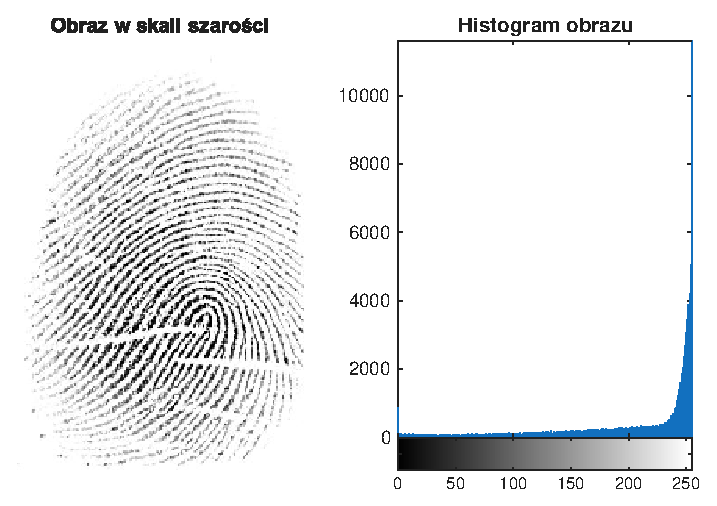
\includegraphics[width=0.7\linewidth]{figures/finger001.eps}\\
    \caption{Obraz wejściowy i jego histogram.\label{Wyniki001}}
\end{figure}

\subsection{Wyrównanie histogramu}
Przeprowadzono operację wyrównywania histogramu w celu poprawy kontrastu (patrz \listingname~\ref{Lab001_l2}):

\lstinputlisting[style= matlabStyle, caption= Wyrównanie histogramu, label=Lab001_l2]{src/Lab001/listing002.m}

\noindent Na \figurename~\ref{Wyniki002} przedstawiono otrzymane rezultaty po wyrównaniu histogramu.

\begin{figure}[H]
    \centering
    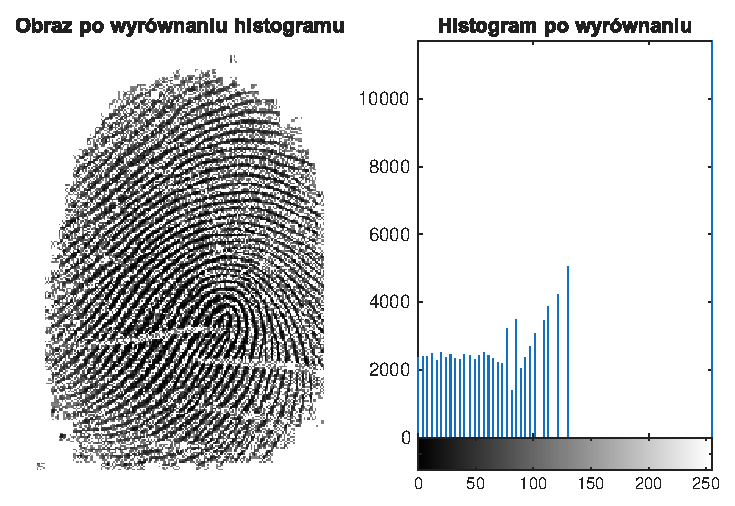
\includegraphics[width=0.7\linewidth]{figures/fingeHistogram.eps}\\
    \caption{Obraz po wyrównaniu i jego histogram.\label{Wyniki002}}
\end{figure}


\section{Wyniki i analiza}
Po przeprowadzeniu analizy histogramu uzyskano następujące wyniki:
\begin{itemize}
    \item Histogram oryginalnego obrazu wykazał skupienie wartości pikseli w wąskim zakresie, co wskazuje na niski kontrast.
    \item Po wyrównaniu histogramu kontrast obrazu uległ poprawie, a wartości pikseli zostały bardziej równomiernie rozłożone.
    \item Metoda Otsu pozwoliła na automatyczne wyznaczenie progu binaryzacji, co umożliwiło efektywne wydzielenie struktur biometrycznych na obrazie.
\end{itemize}

\section{Wnioski}
Na podstawie przeprowadzonych eksperymentów można stwierdzić, że:
\begin{itemize}
    \item Histogram jest przydatnym narzędziem w analizie jakości obrazu biometrycznego.
    \item Wyrównanie histogramu poprawia kontrast i może zwiększać czytelność obrazu.
    \item Segmentacja oparta na histogramie, w szczególności metoda Otsu, pozwala na skuteczne wydzielenie istotnych cech obrazu.
\end{itemize}

\section{Bibliografia}
\begin{itemize}
    \item MATLAB Image Processing Toolbox Documentation \cite{mathworks},
    \item Rafael Gonzalez, Richard Woods, Digital Image Processing Global Edition \cite{gonzalez2017}.
\end{itemize}


% Wyłączenie działania `ulem` na czas bibliografii
\renewcommand{\emph}[1]{\textit{#1}}
% Bibliografia
% Dodanie bibliografi do spisu treści
\addcontentsline{toc}{section}{\textbf{Bibliografia}}
\bibliographystyle{plain}
\bibliography{bibliografia}

% Przywrócenie działania `ulem`
\renewcommand{\emph}[1]{\uline{#1}}

\clearpage
% Dodanie spisu rysunków do spisu treści
\addcontentsline{toc}{section}{\textbf{Spis rysunków}}
\listoffigures
\clearpage

% Dodanie spisu tabel do spisu treści
\addcontentsline{toc}{section}{\textbf{Spis tabel}}
\listoftables
\clearpage


\clearpage

% Dodanie spisu listingow do spisu treści
\addcontentsline{toc}{section}{\textbf{Spis listingów}}
\lstlistoflistings
\clearpage


% \appendix
\chapter*{}
\label{cha:statement-A}
\makeatletter
\addcontentsline{toc}{section}{\textbf{Oświadczenie studenta o samodzielności pracy}}

\noindent
\begin{flushright}
    \begin{minipage}[!h]{10cm}
        Załącznik nr 2 do Zarządzenia nr 228/2021 Rektora Uniwersytetu Rzeszowskiego z dnia 1 grudnia 2021 roku w sprawie ustalenia procedury antyplagiatowej w Uniwersytecie Rzeszowskim
    \end{minipage}
\end{flushright}

\begin{center}
    \vspace*{10mm}
    \noindent  {\textbf{OŚWIADCZENIE STUDENTA O SAMODZIELNOŚCI PRACY} }
    \vspace*{10mm}
\end{center}

\noindent
\dotuline{\hspace{1.3cm}\@author\hspace{1.3cm}}\\ % Linia pozioma
{\small Imię (imiona) i nazwisko studenta }\\

\noindent \@faculty\\

\noindent \dotuline{\hspace{1.4cm}\@degreeprogramme \hspace{1.4cm}}\\
{\small Nazwa kierunku} \\

\noindent \dotuline{\hspace{1.8cm}\@noAlbum\hspace{1.9cm}}\\
{\small Numer albumu}

\begin{enumerate}
    \item Oświadczam, że moja praca projektowa pt.: \@titlePL
          \begin{enumerate}[label=\arabic*)]
              \item została przygotowana przeze mnie samodzielnie*,
              \item nie narusza praw autorskich w rozumieniu ustawy z dnia 4 lutego 1994 roku o prawie autorskim i prawach pokrewnych (t.j. Dz.U. z 2021 r., poz. 1062) oraz dóbr osobistych chronionych prawem cywilnym,
              \item nie zawiera danych i informacji, które uzyskałem/am w sposób niedozwolony,
              \item nie była podstawą otrzymania oceny z innego przedmiotu na uczelni wyższej ani mnie, ani innej osobie.
          \end{enumerate}
    \item Jednocześnie wyrażam zgodę/nie wyrażam zgody** na udostępnienie mojej pracy projektowej do celów naukowo--badawczych z poszanowaniem przepisów ustawy o prawie autorskim i prawach pokrewnych.
\end{enumerate}


\vspace*{10mm}

\noindent
\underline{\hspace{6cm}} \hfill \underline{\hspace{6cm}} \\ % Puste miejsce na miejscowość, data oraz podpis
\hspace*{13mm}(miejscowość, data)  \hspace*{60mm}(czytelny podpis/y studenta/ów)
\vspace*{10mm}

\vfill
\noindent
* Uwzględniając merytoryczny wkład prowadzącego przedmiot \\
** -- niepotrzebne skreślić


\end{document}
